\section{Implementierung}
\label{sec:implementation-analysis}

\subsection{Kontext}

Die bereits existierende Anwendung besteht aus einem Serverseitigen Backend in
Ruby on Rails, der auch die erstellten Webseiten aus Liquid Templates rendert,
und dem in Angular geschriebenen Editor, mit dem die Webseiten erstellt werden.

\subsubsection{Kommunikation via Description Interface}

Server und Client übertragen Daten in der Form von \texttt{JSON} Objekten, die
je Zweck einem Description Interface entsprechen müssen. Ein Description
Interface legt die Felder und Typen der \texttt{JSON} Objekte fest, die diesem Interface
unterliegen. Das Basis Description Interface schreibt folgende Felder vor:

\begin{minted}{json}
{
  "id": "<UUID as string>",
  "name": "<string>",
  "apiVersion": "<unsigned integer>"
}
\end{minted}

\subsubsection{Server: Ruby on Rails}

Rails ist ein in Ruby geschriebenes serverseitiges Framework für
Webanwendungen. Rails mach bestimmte Annahmen darüber was der ``richtige'' Weg
ist, bestimmte Dinge zu tun und was Webanwendungen benötigen und stellt hierfür
Werkzeuge bereit. Rails verfolgt das Model-View-Controller Konzept, aber da die
Anwendung vor Rails Sinatra verwendet hat ist die Logik nicht in Models sondern
in durch den Controller verwendeten Librabies untergebracht. Die Views werden
ebenfalls nicht verwendet. Für den Editor stellen die Controller die vom Angular
Client genutzten \texttt{API} Endpunkte bereit und das eigentliche Frontend wird
in durch die Templating Engine Liquid gerendert.

\subsubsection{Client: Angular 4}

Angular ist eine Platform für Web- und Desktopanwendungen, wobei mit Angular
erstellte Desktopanwendungen Frameworks wie Electron benötigen, die einen
Server, einen kompatiblen Browser und die Daten ``zusammenkleben'' und als
Anwendung ausliefern, im Fall von Electron handelt es sich um Node.js und
Chromium, deren Sicherheitsrelevante Updates eines Updates der Anwendung durch
den Entwickler bedürfen. Im Fall von Webanwendungen liegt es am Nutzer einen
kompatiblen Browser zu verwenden allerdings ist der Nutzer nicht für das
Einspielen von Sicherheitsupdates des Browsers vom Entwickler der Webapp
abhängig und auf den Servern eingespielte Sicherheitsupdates sind sofort für
alle Nutzer gültig.

Angular verwendet Typescript, was zu JavaScript kompiliert wird. Bei
abgeschaltetem JavaScript oder Browsern ohne JavaScript, wie sie unter anderem
von Screenreadern für blinde Nutzer verwendet werden, ist ohne zutun des
Entwicklers nicht mehr als eine leere Seite zu sehen, da alle in Angular
entworfenen Inhalte erst nach dem Laden der Seite durch das Framework in
JavaScript nachgeladen werden.

Angular Anwendungen sind aufgeteilt in Module. In den Modulen befinden sich
Components und Templates. Templates stellen ein Element in der Anwendung dar,
während Components dem Template die dargestellten Daten liefert und auf im
Kontext des Templates auftretende Ereignisse verarbeitet. Dabei kann in einem
Template direkt der Wert einer Eigenschaft der Component referenziert werden,
der dann dort dargestellt und bei Änderung aktualisiert wird und ein Ergeignis
wie onClick direkt mit einer Funktion der Component verbunden werden. Angular
kennt weiterhin Services, die dazu gedacht sind die Kommunikation zwischen
Komponenten zu ermöglichen.

\subsection{Implementationsdetails}

Diese Sektion geht auf die tatsächliche Implementation ein und beschriebt
verschiedene wichtige Aspekte und Herausvorderungen, die dabei eine Rolle
gespielt haben.

\subsubsection{Caching}

Die Bildverwaltung erlaubt es, jederzeit ein Bild zu verändern, ohne dass sich
die \texttt{URL} ändert. Dadurch geht de Client davon aus, dass das in seinem
Cache liegende Bild noch aktuell ist und die neue Version des Bildes nicht
geladen wird, bis das Bild aus dem Cache des Clients gelöscht wurde.

Dieses Verhalten kann umgangen werden, indem die \texttt{URL} für jeden Request
um den aktuellen Zeitstempel als Parameter erweitert wird, führt jedoch dazu,
dass der Cache komplett ausser Kraft gesetz wird. Eine weitere unwirksame
Methode ist das setzen der maximalen Lebensdauer des Bildes im Cache durch den
dafür vorgesehenen \texttt{HTTP} Header, da hierfür der Zeitpunkt der nächsten
Änderung des Bildes bekannt sein müsste. Ohne diese Information ist diese
Methode lediglich eine Balance zwischen den beiden zuvor genannten, aber keine
korrekte Lösung des Problems.

Zur korrekten Lösung des Problems stellt \texttt{HTTP} zwei Header zur
Verfügung: \texttt{ETAG} und \texttt{Last-Modified}. Bei beiden stellt der
Client den Request an den Server, schickt aber den \texttt{Last-Modified} bzw
\texttt{ETAG} Header mit dem vom Server zuletzt übermittelten Wert mit. Der
Server prüft ob der vom Client im Header übermittelte Wert noch aktuell ist und
antwortet mit dem aktuellem Inhalt oder dem Hinweis, dass der vom Client
gecachete Inhalt sich auf Serverseite nicht verändert hat.

\texttt{ETAG} verwendet hierbei eine Checksumme über den Inhalt,
\texttt{Last-Modified} einen Zeitstempel. Im Kontext der Bildverwaltung sind
beide gleich Wirkungsvoll, da jedes Bild im Dateisystem gespeichert wird und
somit der Zeitstempel vom Dateisystem verwaltet und bei Änderungen an der Datei
aktualisiert wird. Die Verwendung der Checksumme setzt voraus, dass für jeden
Request zum Abrufen eines Bildes die Checksumme des Bildes neu berechnet werden
muss. Im Gegensatz zu \texttt{Last-Modified} kann \texttt{ETAG} durch Bitflip
entstandene Bildänderungen feststellen und sie dem Projektautoren schneller
anzeigen und ist resistent gegenüber Manipulation des Zeitstempel im Dateisystem
oder Unregelmäßigkeiteiten in der Systemzeit, allerdings kann ersteres durch
Verwendung hostingtauglicher Festplatten- und Dateisystemkonfigurationen
vermieden werden und letzteres deutet auf einen Hardwaredefekt hin dessen
Mitigation nicht in den Anforderungen an die Bildverwaltung enthalten ist,
während die Manipulation der Zeitstempel externen Eingriff auf durch den
Systemadministrator oder einen Angreifer auf das System bedeutet ersteres
widerspricht der Aufgabe des Systemadministrators und das Verhindern von
letzterem ist sowohl Aufgabe aller am erstellen oder betreiben der Software
beteiligter. \texttt{ETAG} und \texttt{Last-Modified} können auch zusammen
verwendet werden, sodass im Fall einer Veränderung des Bildes das berechnen der
Checksumme entfallen kann, da sich der Zeitstempel bereits unterscheidet. Im
wesentlich häufiger auftretenden Fall des aktuellen Client Caches muss die
Checksumme jedoch weiter berechnet werden.

Die Bildverwaltung verwendet den \texttt{Last-Modified} Header mit dem
Zeitzonenfreien Zeitstempel aus dem Dateisystem, da der zusätzliche Overhead
durch das Berechnen der Checksumme jedes ausgliefertem Bildes keinen
ausreichenden Mehrwert gegenüber der Verwendung des Zeitstempels bietet. Beim
Skalieren der Anwendung auf mehrere nicht unhabhängige Instanzen kann der
\texttt{Last-Modified} Header aus dem Filesystem nicht mehr zuverlässig
verwendet werden ohne dass beim Synchronisieren der Daten die Zeitstempel mit
synchronisiert werden, hier kann die Verwendung des \texttt{ETAG} Headers besser
sein, der Wechsel von \texttt{Last-Modified} zu ETAG ist allerdings trivial.

\subsubsection{API}

Die API stellt verschiedene Routen bereit, die sich in das existierende
Strukturen einfügen, daher sind alle Routen unterhalb von
\mint{ruby}|/api/project/:project_id/image| angesiedelt

\begin{minted}{ruby}
/api/project/:project_id/image
  GET     #gibt die Liste aller Bildmetadaten aus
  POST    #legt ein neues Bild an
/api/project/:project_id/image/:image_id
  GET     #gibt ein Bild aus
  POST    #ersetzt die Bilddatei
  DELETE  #löscht ein Bild inklusive Metadaten
/api/project/:project_id/image/:image_id/metadata
  GET     #gibt die Metadaten eines Bildes aus
  POST    #ersetzt die Metadaten eines Bildes
\end{minted}

Es folgen Ausführungen zu den einzelnen Routen:

\begin{minted}{ruby}
GET /api/project/:project_id/image
\end{minted}

Diese Route liefert eine Liste der Metadaten aller Bilder, die dem Projekt zur
Verfügung stehen. Zur Zeit sind das alle Bilder, die via Bildverwaltung im
Projekt hochgeladen wurden. Geplant ist weiterhin eine Globale Bildverwaltung
deren Bilder in allen Projekten verfügbar sind, sowie nach Implementierung der
Projektvererbung die Bilder aller Projekte in der Vererbungskette. Aus Sicht der
Bildverwaltung macht es daher Sinn alle Projekte die nicht explizit ein anderes
Projekt beerben von einem Speziellen Urprojekt erben zu lassen, in deren
Bildverwaltung die globale Bildersammlung hinterlegt werden, so kann eine
sonderbehandlung in der Bildverwaltung vermieden werden.

\begin{minted}{ruby}
POST /api/project/:project_id/image
\end{minted}

Diese Route wird verwendet um neue Bilder in der Bildverwaltung anzulegen. Es
wird ein Multipart Formular erwartet, bestehend aus dem Bild und den Metadaten.
Da nur der Projektautor in der Lage sein soll das Projekt zu editieren, ist
diese Route, wie der Rest der modifizierenden Editorfunktionen, durch
\texttt{HTTP} Basic Auth abgesichert.

\begin{minted}{ruby}
GET /api/project/:project_id/image/:image_id
\end{minted}

Diese Route liefert das Bild aus, damit es von einem Webbrowser angezeigt werden kann.

\begin{minted}{ruby}
POST /api/project/:project_id/image/:image_id
\end{minted}

Diese Route akzeptiert ein Bild, welches die gespeicherte Bilddatei ersetzt.
Sie ist ebenfalls via Basic Auth abgesichtert.

\begin{minted}{ruby}
DELETE /api/project/:project_id/image/:image_id
\end{minted}

Diese Route wird verwendet um ein Bild inklusive seiner Metadaten zu löschen und
verwendet selbstverständlich Basic Auth.

\begin{minted}{ruby}
GET /api/project/:project_id/image/:image_id/metadata
\end{minted}

Diese Route liefert die Metadaten eines bestimmen Bildes aus.

\begin{minted}{ruby}
POST /api/project/:project_id/image/:image_id/metadata
\end{minted}

Diese abgesichterte Route aktzeptiert einen Satz Metadaten, um den zu dem Bild
gehöhrigen zu ersetzen.

Die versendeten Metadaten entsprechen dem Format des Description Interfaces:

\begin{minted}{json}
{
  "id": "<UUID as string>",
  "name": "<string>",
  "apiVersion": "<unsigned integer>",
  "author-name": "<string>",
  "author-url": "<string>",
  "licence-name": "<string>",
  "licence-url": "<string>"
}
\end{minted}

\subsubsection{Library}
\label{subsec:4-image-library}

Ein Hauptaspekt der Bildverwaltung ist eine Übersicht aller dem Projekt
verfügbaren Bilder und der Möglichkeit die Bilder nach Bildname, Urhebername und
Lizenzname zu filtern. Die Daten stammen aus der \texttt{API} Route, der alle
Bildmetadaten liefert und können sowohl zur besseren Betrachtbarkeit als
Gallerie (siehe Abbildung \ref{fig:impl-image-gallery}) oder zur besseren
Übersicht über die Metadaten als Liste (siehe Abbildung
\ref{fig:impl-image-list}) angezeigt werden.

\begin{figure}
  \centering
  \includegraphics[height=0.95\textheight]{images/screenshot-image-gallery.png}
  \caption{Bildergallerie}
  \label{fig:impl-image-gallery}
\end{figure}

\begin{figure}
  \centering
  \includegraphics[height=0.95\textheight]{images/screenshot-image-list.png}
  \caption{Bildliste}
  \label{fig:impl-image-list}
\end{figure}

Der Upload geschieht über ein der Bildverwaltung untergeordneten Dialog
bestehend aus einem Formular mit Feldern für Name des Bildes, Name des Urhebers,
\texttt{URL} zur Webseite des Urhebers, Name der Lizenz unter der das Bild
verwendet wird, der \texttt{URL} zum Text der Lizenz, sowie dem Dateiupload.

Aus der Übersicht kann jedes Bild einzelnd gelöscht oder bearbeitet werden. Beim
bearbeiten wird ein Dialog ähnlich dem Upload Dialog angezeigt, mit dem
Unterschied, dass uberhalb des Formulars das Bild angezeigt wird und das
Formular aufgeteilt ist in einen Teil für die Metadaten, die mit den aktuellen
Werten vorausgefüllt werden, und einen weiteren Teil um die Bilddatei zu
ersetzen. Jeder Formularteil kann einzelnd abgesendet werden. So kann ein Fehler
in den Metadaten korrigiert werden, ohne dass die Datei erneut hochgeladen
werden muss bzw. die Bilddatei in einem anderen Dateiformat oder anderer
Bildgröße hochzuladen ohne die Metadaten zu verändern.

Die Verwendung von Namen und Url zu einer Lizenz ist auf den ersten Blick eher
unelegant und eine Liste von Lizenzen von der Art Propriätär, Gemeinfrei,
\texttt{CC0}, \texttt{CC-BY}, \texttt{CC-BY-SA}, \texttt{CC-BY-ND},
\texttt{CC-BY-NC}, \texttt{CC-BY-NC-SA} und \texttt{CC-BY-NC-ND} mit bereits
hinterlegten Verweisen auf die Lizenzen und im Falle der \texttt{CC} Lizenzen
den Badges zum Rendern bei der Quellenangabe. Allerdings ist allein die
Auflistung der \texttt{CC} Lizenzen ein Problem. Die aktuelle Fassung der
\texttt{CC} Lizenzen ist \texttt{4.0}, es existieren aber noch ältere Versionen
die immer noch in Verwendung sind. Bei Lizenzen zählt die Version, unter der das
Bild vom Urheber veröffentlicht wurde. Wenn der Urheber das Bild nicht unter der
aktuelleren Version der jeweiligen \texttt{CC} Lizenz neu veröffentlicht hat,
gilt weiterhin die ursprüngliche Version. Die Angabe der falschen Version der
Lizenz bedeutet, dass die Lizenzbedingungen nicht erfüllt sind. Weiterhin
existieren beispielsweise von den \texttt{3.0} Versionen auf verschiedene
Jurisdiktionen portierte Versionen, die wiederum korrekt auseinandergehalten
werden müssen. Weiterhin kann jede der Lizenzen adaptiert werden um zusätzliche
Bedingunen hinzuzufügen. Die Verwaltung der Lizenzliste bedeutet einen großen
Wartungsaufwand, da ständig neue Lizenzen auftauchen können. Außerdem macht die
nötige Anzahl der Lizenzen in der Liste die Auswahl zu umständlich und
verwirrend wenn man die Zielgruppe bedenkt. Da die Zielgruppe außerdem für den
Umgang mit Lizenzen sensibilisiert werden soll ist der Kontakt mit dem Text der
Lizenzen bzw. im Falle der \texttt{CC} Lizenzen wenigstens der Verständliche
Zusammenfassung durchaus zielführend und kann außerdem die Wahrscheinlichkeit
erhöhen dass \texttt{CC} Lizenzen für eigene Werke verwendet werden, da dafür
die Existenz dieser bekannt sein muss.

\subsubsection{Frontendintegration}

Für das Frontend wird die Templating Engine \texttt{Liquid} verwendet. Der
Seiteneditor erzeugt ein Template, in dem Zwei verschiedene Bild Tags enthalten
sein können: einer für grafische Elemente, die in der Quellliste am Ende der
Seite aufgeführt werden, und einer für Abbildungen, denen die Quelle direkt
angehängt ist. Letztres verwendet einen dafür erzeugten Tag displayImageFigure,
der den Tag in eine \texttt{HTML} Figure Umgebung mit dem Bild und der
Quellenangabe rendert.

Für die grafischen Elemente wird ebenfalls ein spezieller Tag verwendet,
allerdings muss dieser nicht nur die \texttt{HTML} Darstellung des Bildes
rendern, sondern auch dafür sorgen, dass das Bild in der Quellenliste aufgeführt
wird. Der Tag muss also einen Seiteneffect auslösen, der das Bild der
Quellenliste hinzufügt, weshalb er \texttt{addToSourceList} heißt. Die
Quellenliste wird durch den Tag \texttt{displaySourceList} gerendert, der am
Ende jeder Seite eingefügt wird.

Es ist im Konzept von \texttt{Liquid} nicht vorgesehen, dass das Rendern eines
Tags einfluss auf darauf folgende Tags hat, weshalb die Quellenliste in einer
globalen Variable gespeichert werden muss. Da mehrere Rendervorgänge
geleichzeitig stattfinden können, die sich allerdings nicht gegenseitig
beeinflussen dürfen, wird für jeden Rendervorgang eine \texttt{UUID} erzeugt,
unter der die Quelliste des Rendervorgangs abgelegt wird bis der Rendervorgang
abgeschlossen ist.

Jedes rendern eines \texttt{addToSourceList} Tags fügt die Metadaten des Bildes
in die Quellliste unter der \texttt{UUID} des Rendervorgangs ein. Dabei wird
gezählt wie oft dieses Bild bereits dargestellt wurde und diese Nummer an die
\texttt{UUID} der Bildes angehängt als \texttt{Id} des \texttt{HTML}
\texttt{img} Elements verwendet, damit die Quellliste auf das Bild verlinken
kann.

Wird die Quellliste gerendert, so werden alle In die Quellliste der
\texttt{UUID} des Rendervorgangs eingetragenen Bildmetadaten nach Urheber und
Bild \texttt{UUID} gruppiert, sodass die Quellliste einen Eintrag je Urheber mit
all seinen Bildern und einen Eintrag je Bild mit allen vorkommen und Link auf
diese enthält. Zum Gruppieren der Urheber wird die Kombination aus Name und
\texttt{URL} des Urhebers verwendet um Urheber gleichen Namens oder Urheber mit
gemeinsamer Webseite auseinanderhalten zu können. Für jedes Bild wird unter dem
Eintrag des Autoren ein Eintrag mit Namen und Lizenz des Bildes angelegt, wobei
dem Namen nummerierte Links angehängt sind, die auf die Vorkommen der Bilder
oben auf der Seite verlinken.

\subsubsection{Seiteneditorintegration}
\label{subsec:4-page-editor}

Der Seiteneditor verfügte bereits über ein Image Element, für das \texttt{src}
und \texttt{alt} wie in HTML üblich befüllt werden konnten. Dieses Element wurde
ersetzt durch eines, bei dem ein Bild aus der Bildverwaltung und die
Darstellungsform auswählbar sind. Dazu wurde eine Angular Komponente geschaffen,
die sowohl an dieser Stelle als auch bei der auswahl des Projektbildes verwendet
wird. Die erste Fassung dieser Komponente ist eine einfache Dropdownliste, in
der die Namen der Bilder aus der Bildverwaltung aufgeführt sind, da derzeit
keine modalen Dialoge zur Verfügung stehen. Sobald sich das ändert, kann
stattdessen ein Auswahldialog wie die Bildübersicht mit den selben
Filteroptionen verwendet werden.

Die folgenden Optionen zur Optimierung der Anzeige sollten in eine eindgültige
Version des Seiteneditors integriert werden. Da dieser Editor aktuell jedoch
überarbeitet wird, war eine Implementierung im Rahmen dieser Thesis nicht mehr
möglich.

Die Bilder in der Bildverwaltung sind nicht notwendigerweise in der Größe
hintelegt, in der sie dargestellt werden sollen. Bei Bildern im SVG Format
wird außerdem die Boundingbox vom Browser nicht als Größe des Bildes verwendet
und somit in voller Bildschirmbreite dargestellt. Deshalb benötigt der
Seiteneditor die Möglichkeit Einfluss auf einige Darstellungsoptionen zu nehmen.

Es sollte möglich sein, entweder die Höhe oder Breite festzulegen. Wenn beide
gleichzeitig festgelegt werden und ein anderes Seitenverhältnis als das des
Bildes gewählt wird, führt dies zu einer Streckung des Bildes wie in Abbildung
\ref{fig:scaling-overview} verdeutlicht.

\begin{figure}
  \begin{subfigure}[b]{0.66\columnwidth}
    
\includegraphics[width=\columnwidth]{images/scale-image-orig.png}
    \caption{Originalbild}
    \label{fig:scaling-original}
  \end{subfigure}
  \begin{subfigure}[b]{0.33\columnwidth}
    
\includegraphics[width=\columnwidth]{images/scale-image-bad1.png}
    \caption{Halbierte Breite}
    \label{fig:scaling-bad1}
  \end{subfigure}
  \begin{subfigure}[b]{0.66\columnwidth}
    \includegraphics[width=\columnwidth]{images/scale-image-bad2.png}
    \caption{Halbierte Höhe}
    \label{fig:scaling-bad2}
  \end{subfigure}
  \begin{subfigure}[b]{0.33\columnwidth}
    \includegraphics[width=\columnwidth]{images/scale-image-good.png}
    \caption{Korrekt auf 50\% skaliert}
    \label{fig:scaling-good}
  \end{subfigure}
  \caption{Skalieren und Strecken von Bildern}
  \label{fig:scaling-overview}
\end{figure}

Desweiteren ist die Skalierungsmethode eine wichtige Option. Für reguläre Bilder
sollte zum Schrumpfen der Bilder eine qualitativ hochwertige Interpolation
verwendet werden während das vergrößern von Pixelart via Nearest Neighbor
geschehen sollte, da sonst die für Pixelart übliche harten Kanten (siehe
Abbildung \ref{fig:pixelart-scaled-good}) in weiche Kanten umgewandelt werden
und das Bild den Eindruck vermittelt unscharf zu sein (siehe Abbildung
\ref{fig:pixelart-scaled-bad}). Da nach dem Erzeugen des Templates durch den
Editor das Bild in der Bildverwaltung verändert werden kann, kann die richtige
Interpolationsmethode nicht automatisch berechnet und im Template abgelegt
werden, daher muss wie Wahl der korrekten Interpolationsmethode dem
Seitenautoren überlassen werden.

\begin{figure}
  \begin{subfigure}[b]{\columnwidth/2}
    \includegraphics[width=\columnwidth]{images/pixelart-scaled-bad.png}
    \caption{Hochwertige Interpolationsmethode}
    \label{fig:pixelart-scaled-bad}
  \end{subfigure}
  \begin{subfigure}[b]{\columnwidth/2}
    
\includegraphics[width=\columnwidth]{images/pixelart-scaled-good.png}
    \caption{Nearest Neighbor}
    \label{fig:pixelart-scaled-good}
  \end{subfigure}
  \caption{(Un)Tauglichkeit guter Skalierungsmethode für Pixelart}
  \label{fig:pixelart-scaling-overview}
\end{figure}

Diese Eigenschaften sowie die Auswahl des Darstellungstyps müssen sowohl für das
Image Element als auch für Tabellen in denen Bilder angezeigt werden auswählbar
sein.

Das Image Element soll weiterhin in der Lage sein sich in Fließtext zu
integrieren, daher ist für das Image Element zusätzlich die Auswahl des Float
Typs mit den Optionen \texttt{left}, \texttt{right} and \texttt{none} notwendig.
Wollte man kleine Bilder im Fließtext unterbringen so käme noch die Auswahl des
Display Typs zwischen \texttt{block} und \texttt{inline-block} hinzu, allerdings
kann das Image Element derzeit nicht innerhalb eines Paragraphen verwendet
werden, daher entfällt diese Auswahl.

Diese Features konnten allerdings nicht mehr als Teil dieser Thesis
implementiert werden, daher existiert hier nur die Beschreibung dessen was sein
sollte.

\subsubsection{Datenbankintegration}
\label{subsec:4-database-integration}

\begin{figure}
  \centering
  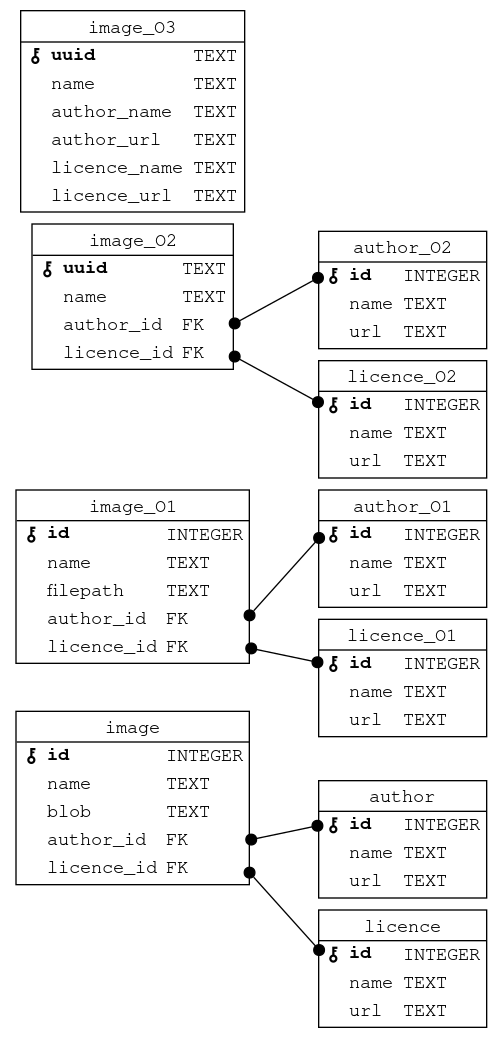
\includegraphics[height=0.95\textheight]{images/image_database_schemas.png}
  \caption{Datenbankschema mit Denormalisierungsschritten}
  \label{fig:database-schema-optimization}
\end{figure}

Mit einer Datenbank, die die Bilddateien in Datenbank in den Tabellen speichern
kann ist der erste Ansatz davon gebrauch zu machen. Daraus resultiert das in
Abbildung \ref{fig:database-schema-optimization} Schema
bestehend aus der Tabellengruppe \texttt{image}, \texttt{author} und
\texttt{licence} wie in der Abbildung dargestellt. Dies bedarf jedoch einem
Datenbankzugriff für jedes darzustellende Bild, so dass das Schema statt dem
Blob den Pfad zum Bild im Dateisystem beinhalten sollte, wie in
\texttt{image\_O1}, \texttt{author\_O1} und \texttt{licence\_O1} dargestellt. Da
die Bilder durch ihre UUID bereits eindeutig identifiziert werden ist die
Verwendung einer datenbankeigenen Id reduntant, außerdem kann die UUID verwendet
werden um den Pfad der Bilddatei im Dateisystem zu berechnen, solange dieser
systematisch in Abhängigkeit von der UUID erzeugt wird, sodass das Speichern des
Dateipfads ebenfalls reduntant ist. Das Ergebnis ist in der Tabellengruppe
\texttt{image\_O2}, \texttt{author\_O2} und \texttt{licence\_O2} zu sehen. Da
das Abrufen aller Metadaten die häufigste Operation ist, lohnt es sich die
Tabellengruppe zu denormalisieren um diese Operation ohne das zusammenführen
mehrer Tabellen auszuführen zu können. Das Schema der resultierenden Tabelle ist
in der Abbildung unter \texttt{image\_O3} zu sehen. Da das Projekt zum aktuellen
Zeitpunkt noch Sqlite verwendet, ist diese Tabelle in eine JSON Datei im
Bilderordner ausgelagert um die Last auf der Datenbank zu verringern.

In der derzeitigen Implementierung werden Bild-UUIDs in der Datenbank in
regulären Text Feldern gespeichert und immer wenn der Wert eines Feldes dem
regulären Ausdruck einer UUID genügt wird ein Bild gerendert. Wenn Wechsel der
Datenbanktechnologie auf PostgreSQL erfolgt ist, kann ein Datentyp ImageId
angelegt werden, dessen Wertebereich auf UUIDs beschränkt ist, sodass die
Prüfung beim Rendervorgang auf den Datentyp der Spalte beschränkt werden kann
und die Prüfung auf korrekte Struktur der UUID auf den Zeitpunkt des Einfügens
in die Datenbank verschoben werden und der Autor einer Datenbank kann UUIDS in
Tabellen rendern lassen, ohne dass versucht wird ein Bild an dieser Stelle
darzustellen.

\subsection{Containerisierung}
\label{subsec:4-containerization}

Es wurde ein Entwicklungs und ein Test Docker Image geschaffen, die zur Nutzung
durch die Entwickler bzw. das verwendete CI-System Bitbucket Pipelines gedacht
sind. Beide Basieren auf einem gemeinsamen Basisimage, auf dem auch das
Produktivimage basieren soll. Sämtliche Arbeit an dem Projekt im Kontext dieser
Thesis wurde unter Zuhilfenahme des Entwicklungs Docker Images auf einem Debian
bzw. Archlinux Host durchgeführt und der aktuelle Stand hat sich als
praxistauglich erwiesen und ermöglichte den Problemlosen Wechsel des
Entwicklungsgeräts ohne Aufwand jenseits der eigentlichen
Betriebssysteminstallation. Desweiteren wurde das Entwicklungs Image kurz vor
Abgabe der Thesis unter MacOS zum Einsatz gebracht, allerdings zu kurz um die
Stabilität auf dieser Platform bereits zu bestätigen. Das Test Image wird seit
Fertigstellung von Bitbucket Pipelines benutz und führt alle vorhandenen Tests
für jeden Commit aus.

Die Images sollten ursprünglich auf Alpine Linux basieren, um besonders klein zu
sein, allerdings ließ es die aktuelle Situation der Packete im
Packetmanagementsystem nicht zu alle benötigten Abhängigkeiten in der Korrekten
Version gleichzeitig zu installieren ohne größeren Aufwand zu treiben, weshalb
vorerst das Archlinux Base Development Docker Image verwendet wird, was leider
um den Faktor hundert größer ist, sich aber deutlich einfacher Einrichten ließ.
Es ist geplant den Wechel auf Alpine Linux durchzuführen, sobald dies möglich ist.

Es wurde ein Makefile geschaffen, um die Nutzung durch Entwickler die weder mit
Docker noch Docker-Compose vertraut sind zu vereinfachen, und ihnen sowohl
ermöglicht das Projekt schnell in Betrieb zu nehmen, als auch aus dem Makefile
zu lernen. Das Makefile enthält Targets um die Entwicklungsumgebung zu starten
und zu stoppen, die Tests auszuführen, die Images von Dockerhub herunterzuladen,
die Images neu zu bauen, die gebauten Images auf Dockerhub hochzuladen.

Das Produktivimage wurde bisher nicht fertiggestellt, da derzeit noch keine im
Produktivbetrieb einsetzbare Version von SQLino existiert, die darin
ausgeliefert werden könnte, daher wurde die Fertigstellung mit einer niedrigen
Priorität versehen und konnte nicht in der gegebenen Zeit fertiggestellt werden.

%%% Local Variables:
%%% mode: latex
%%% TeX-master: "thesis"
%%% End:
